\begin{enumerate}[label=\thesubsection.\arabic*.,ref=\thesubsection.\theenumi]
\numberwithin{equation}{enumi}

\item A second-order LTI system is described by the following state equations:
\begin{align}
\label{eq:qe1}
\frac{\partial x_1(t)}{\partial t} - x_2(t) = 0
\end{align}
\begin{align}
\label{eq:qe2}
\frac{\partial x_2(t)}{\partial t} + 2x_1(t) + 3x_2(t) = r(t)
\end{align}

where $x_1(t)$ and $x_2(t)$ are the two state variables and r(t) denotes the input. The output c(t) = $x_1(t)$.

\item Identify the type of system employing the state space model. 

\solution Any state space model is represented by:
\newline State Equation:
\begin{align}
\dot{X} = AX + BU
\end{align}
\newline Output equation:
\begin{align}
Y = CX + DU
\end{align}
Comparing these with \eqref{eq:qe1} and \eqref{eq:qe2} we get the state matrices as,
\begin{align}
    A = \myvec{0&1\\-2&-3}
\end{align}
\begin{align}
    B = \myvec{0\\1}
\end{align}
\begin{align}
    C = \myvec{1&0}
\end{align}
\begin{align}
    D = 0
\end{align}

\item Solving for the system transfer function $H(s)$.

\solution The transfer function for the state space model is given by:
\begin{align}
H(s) = C(sI - A)^{-1}B + D
\end{align}
\begin{align}
& = \frac
{
\myvec{1&0}\myvec{s+3&1\\-2&s}\myvec{0\\1}
}
{
s(s+2\beta) + \alpha
}
\end{align}
\begin{align}
\implies H(s) = \frac{1}{s^{2}+3s+2}
\end{align}
Therefore, poles of transfer function are given by:
\begin{align}
s = -1
\end{align}
\begin{align}
s = -2
\end{align}
Since the poles are negative real and distinct, the system is an OVERDAMPED SYSTEM.

\item Perform the calculations to obtain the output as well as transfer function from state space matrices:

\solution The following code:

\begin{lstlisting}
\small{https://github.com/neildhami18/EE2227/blob/master/codes}
\end{lstlisting}

\item Natural response and comparison plot.
\newline
\solution Natural response:
\begin{align}
    h(t) = L^{-1}(H(s)) = e^{-t} - e^{-2t}
\end{align}
\solution Comparison plot:
\newline 
Consider the system with same natural frequency , but different damping ratios. The figure below shows a comparative plot of natural response between all the three types of systems.
\newline
\begin{figure}
\centering
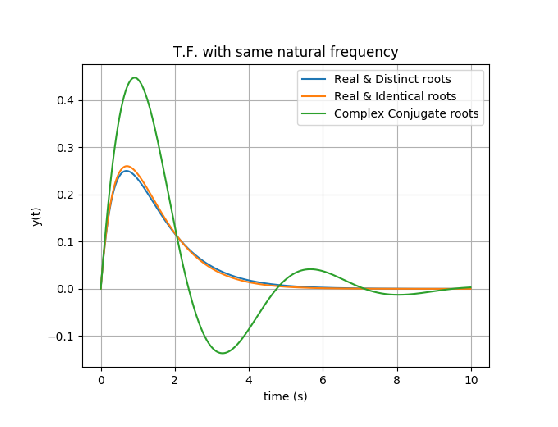
\includegraphics[width=\columnwidth,height=4cm]{test.eps}
\end{figure}
%\begin{figure}[!ht]
%	\begin{center}
%\includegraphics[width=\columnwidth]{./figs/ee18btech11011.eps}		
%	\end{center}
%\caption{}
%\label{fig:ee18btech11011}
%\end{figure}

\end{enumerate}
